\chapter{Core}

\pulpino supports both the OpenRISC \orion core and the \riscv \rvcore. The two
cores have the same external interfaces and are thus plug-compatible.

The core use a very simple data and instruction interface to talk to data and
instruction memories. To interface with AXI, a core2axi protocol converter is
instantiated in \pulpino.

The core is connected via a debug interface to the advanced debug unit which
allows in-circuit debugging.

The core supports performance counters. Those are mainly used for counting core
internal events like stalls, but it is possible to count core-external events
as well. For this purpose there is the \texttt{ext\_perf\_counters\_i} port where
arbitrary events can be attached. The core then increases its internal
performance counter for this event type every time a logic high is seen on this
port.

\begin{figure}[ht]
	\centering
  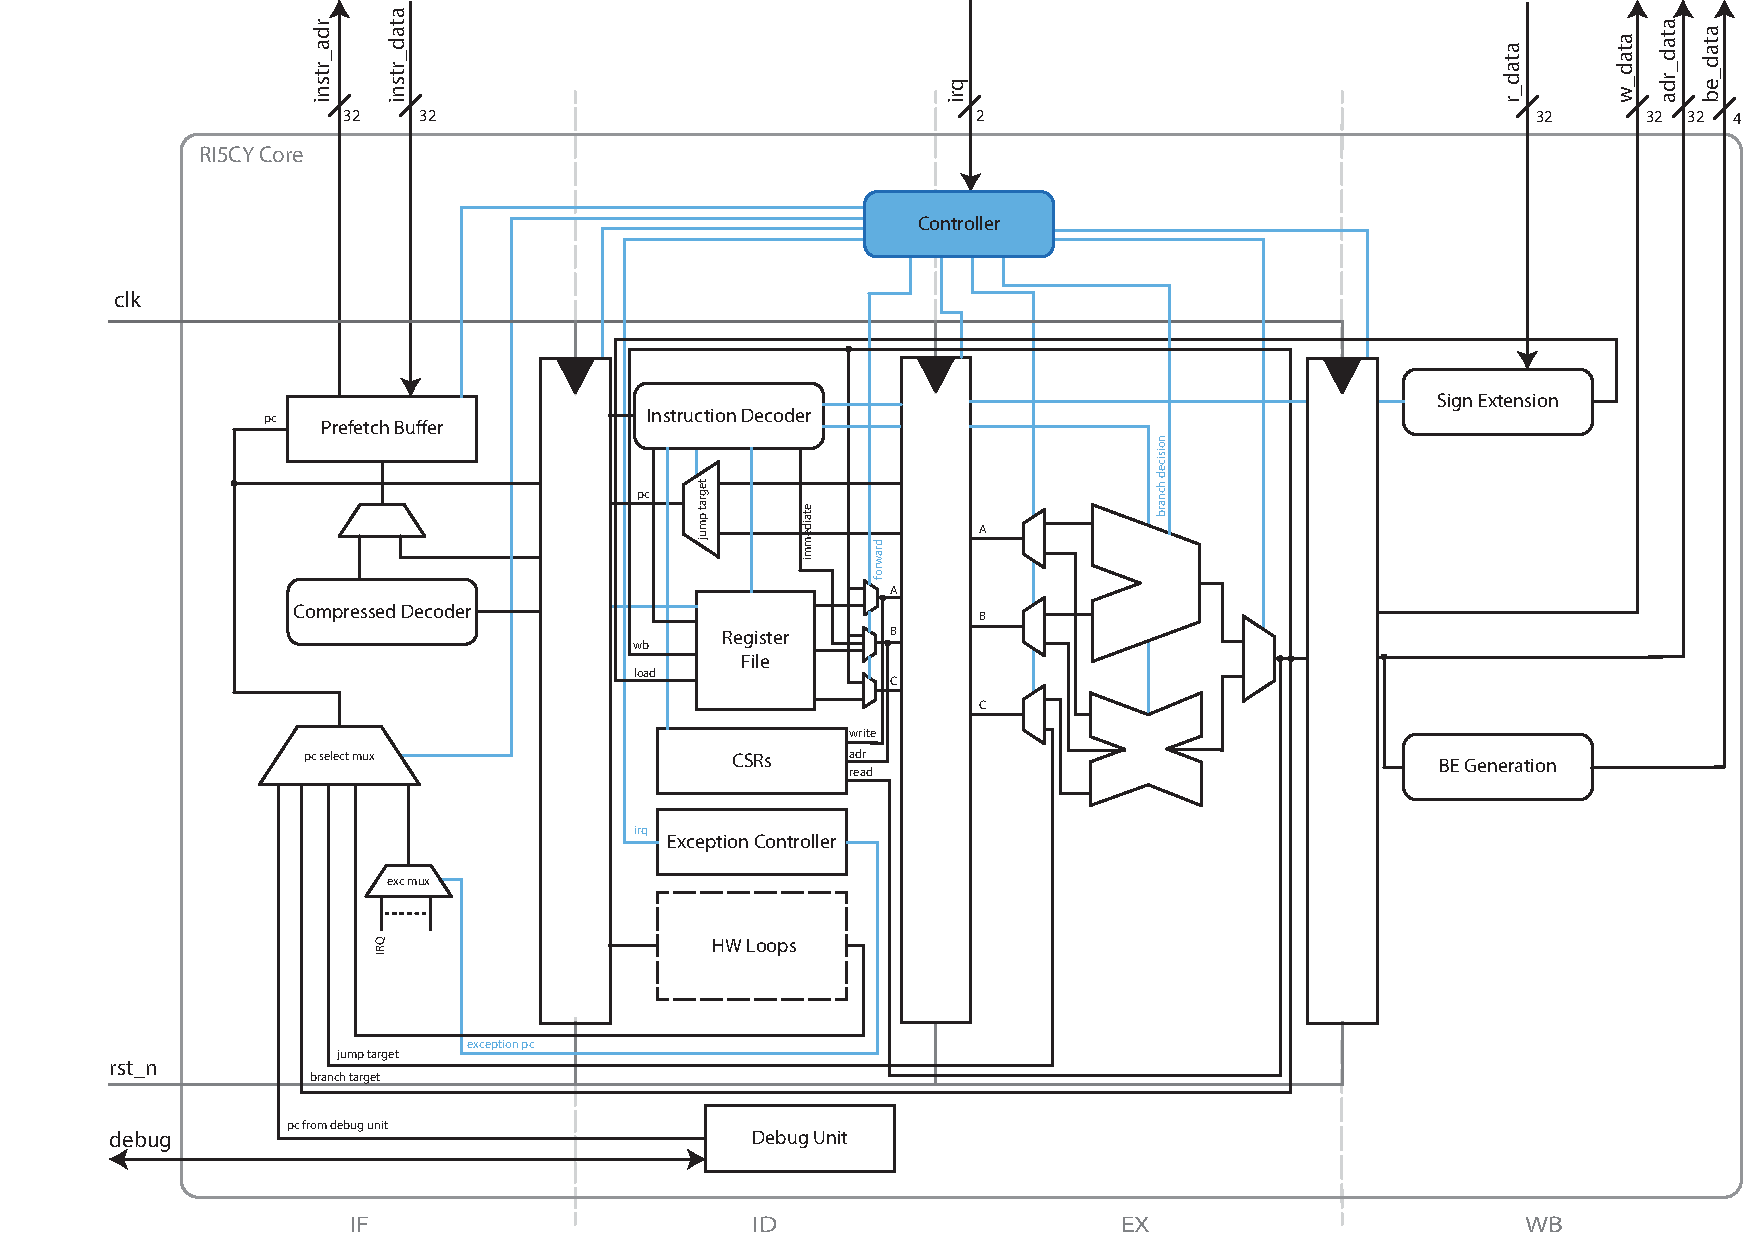
\includegraphics[width=1.5\textwidth, angle=90]{./figures/riscv_arch}
	\caption{RISC V core overview}
	\label{fig1}
\end{figure}